\renewcommand{\thechapter}{2}
\chapter{Theory of \texorpdfstring{$\beta\beta 0\nu$}{Neutrinoless Double-Beta} Decay}
\label{ch:BB0NTheory}

Toward the end of the 1990s neutrinos were conclusively proven to possess a non-zero mass.  Subsequent effort has been directed toward understanding the absolute scale of neutrino mass and the nature of the interaction which causes it.  Neutrinoless double-beta ($\beta\beta 0\nu$) decay, if it occurs, would provide a window onto both questions.  This chapter presents the theoretical motivations for searching for $\beta\beta 0\nu$ decay.  Section~\ref{sec:TheoryStandardDoubleBeta} describes the closely-related two-neutrino double-beta ($\beta\beta 2\nu$) decay which is allowed in the standard model.  Section~\ref{sec:TheoryNeutrinolessDoubleBeta} defines $\beta\beta 0\nu$ decay and reasons for hypothesizing its occurrence.  Considerations and challenges in nuclear physics are described in section~\ref{sec:NuclearMatrixCalculations}.  The parametrization of the neutrino sector is provided in section~\ref{sec:NeutrinoFlavorPhysics}.  Section \ref{sec:ParticlePhysicsConstraints} summarizes constraints on neutrino masses which can be obtained from observations of single-$\beta$ decay and cosmology, and section \ref{sec:NucPhysConstraintsFromBB0N} describes in detail the considerations and challenges involved in searching for $\beta\beta 0\nu$ decay.  The reader will obtain a general understanding of the state of the field before continuing on to the details of the EXO-200 detector in chapter~\ref{ch:EXO200Detector}.

\begin{figure}
\begin{center}
\includegraphics[keepaspectratio=true,width=2in]{Avignone_fig02a.eps}
\end{center}
\renewcommand{\baselinestretch}{1}
\small\normalsize
\begin{quote}
\caption{Feynman diagram for $\beta\beta 2 \nu$ decay.  The reaction products are equivalent to two $\beta$ decays in succession, but this reaction can sometimes occur even if a single $\beta$ decay would be energetically forbidden.  Figure from~\cite{RMPbb0n}.}
\label{fig:FeynmanBetaBeta2Nu}
\end{quote}
\end{figure}
\renewcommand{\baselinestretch}{2}
\small\normalsize

\section{Double-Beta Decay}\label{sec:TheoryStandardDoubleBeta}

Standard-model two-neutrino double beta ($\beta\beta 2\nu$) decay is the result of the particle interaction
\begin{equation}\label{eqn:bb2n_decay_reaction}
2d \rightarrow 2u + 2e^- + 2\bar{\nu}_e
\end{equation}
mediated by $W^-$-exchange, as depicted in Figure~\ref{fig:FeynmanBetaBeta2Nu}.  It is effectively the simultaneous occurrence of two beta ($\beta$) decays from the same nucleus.

Because $\beta\beta 2\nu$ decay is of a second-order weak interaction, it has a remarkably slow rate compared to most $\beta$ decay processes.  Although many nuclei are expected to decay by $\beta\beta 2\nu$, the process is thoroughly masked by conventional $\beta$ decay in most of them.  In most cases, we can only hope to detect $\beta\beta 2\nu$ decay in isotopes where $\beta$ decay is forbidden or highly suppressed.

An example of an isotope for which $\beta$ decay is highly suppressed is $^{48}_{20}$Ca.  The ground state of $^{48}_{20}$Ca has zero units of angular momentum, whereas its single-$\beta$-decay daughter product $^{48}_{21}$Sc has six units of total angular momentum in its ground state, and is thus highly suppressed by angular momentum conservation.  In contrast, $^{48}_{22}$Ti has zero units of total angular momentum, making $\beta\beta 2\nu$ decay of $^{48}_{20}$Ca permitted by angular momentum and energy considerations, and as a result the $\beta\beta 2\nu$ decay mode of $^{48}_{20}$Ca dominates~\cite{MyNuclearPhysicsBook}.

In most $\beta\beta 2\nu$ candidates, single $\beta$ decay is forbidden by energy conservation.  It is well-known that nuclei minimize their energy by arranging similar nucleons to have overlapping wavefunctions~\cite{MyNuclearPhysicsBook}.  Thus, isotopes with an even number of protons and an even number of neutrons will have less nucleon-pairing potential energy than an isotope with either an odd number of protons or an odd number of neutrons, which in turn will have less nucleon-pairing potential energy than an isotope with an odd number of protons and an odd number of electrons.

\begin{figure}
\begin{center}
\includegraphics[keepaspectratio=true,width=\textwidth]{scripts/LevelDiagram.png}
\end{center}
\renewcommand{\baselinestretch}{1}
\small\normalsize
\begin{quote}
\caption{Energy diagram of isotopes with atomic mass $A=136$.  The energies $\Delta E$ are the binding energies of the atom, compared to the bare masses of the same nuclei.  Values are from~\cite{AtomicMassEvaluation}.}
\label{fig:LevelDiagram}
\end{quote}
\end{figure}
\renewcommand{\baselinestretch}{2}
\small\normalsize

A typical nuclear energy level diagram is shown in figure~\ref{fig:LevelDiagram} for the $A=136$ isobar: Xenon, Barium, Cerium, and Neodynium are even-even isotopes, and have systematically lower energies than the odd-odd isotopes Iodine, Cesium, Lanthanum, and Praseodymium.  For this particular isobar, we can see that Xenon is energetically forbidden from single-$\beta$ decaying to Cesium because the odd-odd isotope of Cesium has slightly more potential energy than the even-even isotope of Xenon. As a result, the primary mode of decay of Xenon-136 will be $\beta\beta 2\nu$ decay to Barium-136.  Similarly, the primary mode of decay of Cerium-136 will be by double-electron-capture with neutrino emission ($\epsilon\epsilon 2\nu$) to Barium-136.  Many of the same implications of $\beta\beta 0\nu$ decay also apply to the theorized $\epsilon\epsilon 0\nu$ decay; however, in practice the expected rates for these decays will be lower than the rates for $\beta\beta 0\nu$ decay, so we will not consider them further in this work.

\section{Neutrinoless Double-Beta Decay}\label{sec:TheoryNeutrinolessDoubleBeta}

The detection and study of $\beta\beta 2\nu$ decay provides an opportunity to test a class of nuclear matrix element computations; however, it does not violate any fundamental symmetries and is, in this sense, a mundane prediction of the Standard Model.  The primary appeal of isotopes which undergo $\beta\beta 2\nu$ decay is the opportunity these isotopes provide to probe the nature of neutrinos.

It has been suggested as early as 1937 that neutrinos could possess mass through a neutrino-antineutrino interaction, provided that the neutrino is its own antiparticle~\cite{Majorana}.  The theorized Majorana interaction comes from Lagrangian terms of the form (for each of three neutrino eigenstates)
\begin{align}
\mathcal{L}_{Maj}&= \begin{aligned}[t]
 & -\frac{m_{L}}{2} \left( \overline{\Psi_L^c} \Psi_L^{} + \overline{\Psi_L^{}} \Psi_L^c \right)\\
 & -\frac{m_{R}}{2} \left( \overline{\Psi_R^c} \Psi_R^{} + \overline{\Psi_R^{}} \Psi_R^c \right),
\end{aligned}
\end{align}
where the superscript-$c$ represents charge conjugation.  (This is the reason that Majorana mass terms are only possible for a chargeless lepton.)  The masses $m_L$ and $m_R$ may be chosen independently; since there has never been an observation of right-handed neutrinos or left-handed anti-neutrinos, it is possible that $m_R = 0$ and that the fields $\Psi_R^{}$ and $\Psi_R^c$ do not exist in nature~\cite{RMPbb0n}.

\begin{figure}
\begin{center}
\includegraphics[keepaspectratio=true,width=2in]{Avignone_fig02b.eps}
\end{center}
\renewcommand{\baselinestretch}{1}
\small\normalsize
\begin{quote}
\caption{Feynman diagram for $\beta\beta 0 \nu$ decay.  A virtual neutrino mediates the exchange.  This is only possible if $\overline{\nu}_R$ can flip its handedness to $\nu_L$, and the interaction that induces this parity change also generates neutrino mass.  Figure from~\cite{RMPbb0n}.}
\label{fig:FeynmanBetaBeta0Nu}
\end{quote}
\end{figure}
\renewcommand{\baselinestretch}{2}
\small\normalsize

If neutrinos do have Majorana mass interactions, then any isotope that undergoes $\beta\beta 2\nu$ decay can also undergo the related process $2d \rightarrow 2u + 2e^-$, depicted in Figure~\ref{fig:FeynmanBetaBeta0Nu}, in which the two outgoing neutrinos in $\beta\beta 2\nu$ decay are replaced by one virtual neutrino.  We can interpret this as a mixing interaction between a left-handed neutrino and a right-handed antineutrino; this is only possible if neutrinos are Majorana particles.  We refer to the standard process as two-neutrino double beta ($\beta\beta 2\nu$) decay and the novel process as neutrinoless double beta ($\beta\beta 0\nu$) decay.

The tree-level diagram for $\beta\beta 0\nu$ has one additional interaction vertex compared to $\beta\beta 2\nu$ decay, and as a result we would expect it to occur at an even slower rate.  However, the more immediate consequence of $\beta\beta 0\nu$ decay is that lepton number conservation is violated.  The lepton number changes by two units corresponding to the creation of two leptons with no balancing anti-leptons.  Numerous theories have suggested other plausible modes of lepton number non-conservation~\cite{ProtonDecay,MuonToPositron}, but none have yet reported a positive result.  In the conventional Standard Model with massless neutrinos, lepton number conservation is an accidental symmetry~\cite{LeptonConservation}, but in a model with massive neutrinos there may no longer be any reason \textit{a priori} to expect conservation or non-conservation of lepton number.

\begin{figure}
\begin{center}
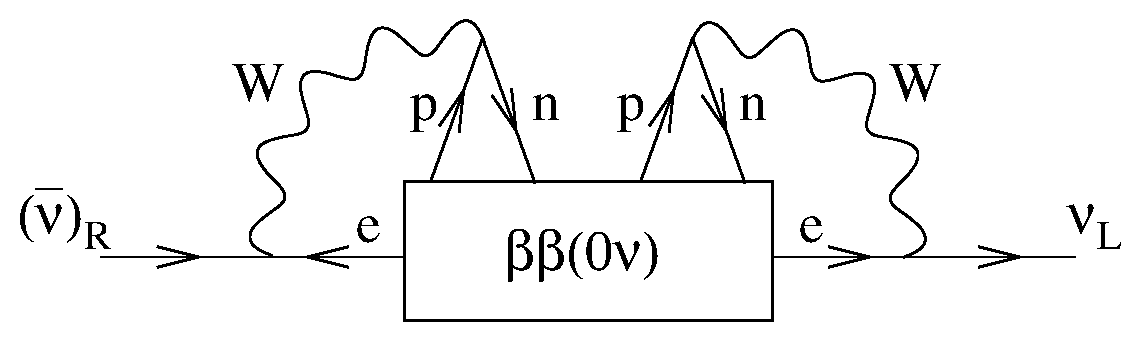
\includegraphics[keepaspectratio=true,width=\textwidth]{Avignone_fig03.eps}
\end{center}
\renewcommand{\baselinestretch}{1}
\small\normalsize
\begin{quote}
\caption{Even without any assumptions about the mechanism which leads to $\beta\beta 0\nu$ decay, we can use that process to generate an effective neutrino mass as a higher-order process.  Figure from~\cite{RMPbb0n}.}
\label{fig:FeynmanBetaBeta0NuImplication}
\end{quote}
\end{figure}
\renewcommand{\baselinestretch}{2}
\small\normalsize

It is worth noting that the interaction term above assumes no mediating particles in the mechanism, whereas it is possible that $\beta\beta 0\nu$ could be mediated by some higher-order interaction terms.  However, if $\beta\beta 0\nu$ decay is observed, it leads very generally to a conclusion that neutrinos have an \emph{effective} Majorana mass interaction~\cite{BlackBoxTheorem}.  We can see this by embedding the $\beta\beta 0\nu$ process into a higher-order one, as shown in figure~\ref{fig:FeynmanBetaBeta0NuImplication}.  Regardless of the details of how $\beta\beta 0\nu$ occurs, its existence would necessarily generate an effective neutrino mass as a higher-order process.

\begin{figure}
\begin{center}
\includegraphics[keepaspectratio=true,width=\textwidth]{halflife_vs_year.pdf}
\end{center}
\renewcommand{\baselinestretch}{1}
\small\normalsize
\begin{quote}
\caption{$\beta\beta 0\nu$ half-life limits versus the year of the limit.  Colors indicate which isotope is under study.  Open circles indicate experiments which have not yet concluded data-taking.  Data is from ~\cite{
PhysRevC.85.045504,PhysRevLett.110.062502,bb0nSearch2012,PhysRevLett.111.122503,
KlapdorDissent,PhysRevLett.83.41,PhysRevC.59.2108,PhysRevD.65.092007,Andreotti2011822,PhysRevC.78.035502,
PhysRevLett.95.142501,Arnaboldi2004260,Baudis1997219,PhysRevLett.95.182302,NEMO2004,NEMO3-2013-100Mo,
doi:10.1142/S0217732390001475,Bernabei200223,Balysh1994176,0954-3899-17-S-014,Arnaboldi2003167,
1112.0859,Baksan2006Gavriljuk,Luescher1998407,Alessandrello1992176,Alessandrello1994519,Alessandrello1998156,
Alessandrello200013,PhysRevD.48.1009,PhysRevLett.59.419,Bellotti1991193,Bellotti1989209,BellottiMilano1986,
Bellotti1984450,Bellotti198372,BellottiMilano1982,PhysRevD.45.2548,PhysRevC.63.065501,0305-4616-13-6-012,
Ejiri199685,Ejiri199117,PhysRevC.55.474,PhysRevLett.71.831,PhysRevLett.63.1671,Fisher1989257,
PhysRevLett.50.721,PhysRevC.34.666,PhysRevLett.53.141,PhysRevD.51.2090,Forster1984301,PhysRevC.56.2451,
Barabash1989273,Fiorini1967602,Fiorini1973,Barabanov:1986iz,Vasilev:1990gi,PhysRevC.38.895}.}
\label{fig:Halflife_vs_year}
\end{quote}
\end{figure}
\renewcommand{\baselinestretch}{2}
\small\normalsize

It has long been clear that appealing extensions to the Standard Model can be built around neutrinos with Majorana mass; see eg. the introduction in 1980 of the see-saw mechanism in~\cite{PhysRevLett.44.912}, where the naturalness of the neutrino mass scale is addressed by hypothesizing $m_R$ is inversely related to $m_L$ and $m_L \ll m_R$.  The motivation to search for $\beta\beta 0\nu$ decay became stronger when neutrinos were proven to have mass, particularly by the definitive proof of the oscillation of atmospheric neutrinos in~\cite{SuperK}.  As a result, the number of experiments searching for $\beta\beta 2\nu$ decays increased rapidly during this time period; figure~\ref{fig:Halflife_vs_year} shows a collection of $\beta\beta 0\nu$ half-life limits obtained versus year, colored by the isotope under study.  The search for $\beta\beta 0\nu$ has by now evolved into a highly competitive field, in which the isotopes $^{130}$Te, $^{76}$Ge, and $^{136}$Xe are particularly dominant but searches are also being actively pursued in many other isotopes.

\section{Double-beta Decay Nuclear Matrix Calculations}\label{sec:NuclearMatrixCalculations}

If the mechanism of $\beta\beta 0\nu$ decay is a tree level neutrino mass term as shown in figure~\ref{fig:FeynmanBetaBeta0Nu}, then the rate of $\beta\beta 0\nu$ decay will also reflect the magnitude of the neutrino mass parameters.  To specify this relation precisely we need an understanding of the nuclear physics of the decaying isotope.  This section will identify the relevant quantities which must be computed and provide a survey of the computational approaches to estimating them.

For a tree-level Majorana interaction we can write the partial half-life $T^{0\nu}_{1/2}$ of an isotope which undergoes $\beta\beta 0\nu$ decay can be described by
\begin{equation}\label{eqn:HalfLifeMatrixElementEqn}
\left[T^{0\nu}_{1/2}\right]^{-1} = G_{0\nu}(Q_{\beta\beta}, Z) \left| M_{0\nu}\right|^2 \left< m_{\beta\beta} \right>^2,
\end{equation}
where $G_{0\nu}(Q_{\beta\beta}, Z)$ is a phase-space factor coming from the range of possible output states, $M_{0\nu}$ is a nuclear matrix element, and $\left< m_{\beta\beta} \right>$ is the effective $\beta\beta 0\nu$ neutrino mass which will be defined in section~\ref{sec:NucPhysConstraintsFromBB0N}.

The two factors $G_{0\nu}(Q_{\beta\beta}, Z)$ and $M_{0\nu}$ will be computed by quite different methods, and it is common to draw nuclear matrix elements and phase factors from different sources.  However, this must be done carefully: scaling factors can be absorbed from one into the other, and if nuclear matrix elements and phase factors are calculated using different conventions, the result of combining them will not be correct.

For example, in early calculations, the nuclear matrix element and phase-space factor were generally computed in units of $\mathrm{fm}^{-1}$ and $\mathrm{yrs}^{-1} \mathrm{fm}^2$, respectively.  Starting in the mid-1980s common practice shifted to multiply the nuclear matrix element by the nuclear radius $R_0 \propto A^3$, where $A$ is the number of nucleons, and divide the phase-space factor by $R_0^2$, making the nuclear matrix element unitless and the phase-space factor have units of $\mathrm{yrs}^{-1}$.  This new convention is fine itself, but care must be taken that the nuclear radius used in both calculations is the same, whereas for many years different authors might choose $R_0 = 1.1 A^3$ fm or $R_0 = 1.2 A^3$ fm without specifying that choice~\cite{PhysRevC.73.028501}.  Modern practice is now that $R_0$ is explicitly specified in any nuclear matrix or phase-space factor calculations.  Similar differences in convention can occur from the choice of whether the fourth power of the axial vector current $g_A^4$ should be included with the phase space factor, nuclear matrix element, or separately as its own factor of equation~\ref{eqn:HalfLifeMatrixElementEqn}, and one must be careful to understand the chosen conventions before combining results from different sources~\cite{PhysRevC.87.014315}.

The phase-space factor $G_{0\nu}(Q_{\beta\beta}, Z)$ accounts for the phase space of the end-state of $\beta\beta 0\nu$ decay.  This includes two outgoing electrons and an outgoing nucleus.  The mass of the outgoing nucleus is always much larger than the masses of the neutrinos, so nearly all momentum will be carried by the two electrons.  Each contributes a phase space integral of the form $\int_0^{p_{max}} \mathrm{d}\cdot p pE$, which individually contribute a factor proportional to $p_{max}^3$.  Considering the system in the rest frame of the incoming nucleus, the sum of the two electron momenta are constrained to be equal to zero, so the combined phase space integral for both electrons is proportional to
\begin{equation}
\int_0^{p_{max}} \mathrm{d}p_1 p_1E_1 \int_0^{p_{max}} \mathrm{d}p_2 p_2E_2 \delta(p_2-p_1) \propto p_{max}^5.
\end{equation}
As a result, the phase space factor $G_{0\nu}(Q_\beta\beta, Z)$ of $\beta\beta 0\nu$ decay will be proportional to $Q^5$, where $Q$ is the total energy of the decay~\cite{mohapatra1998massive}.  The strong dependence of $G_{0\nu}(Q_\beta\beta, Z)$ on $Q$ means that isotopes which have high $Q$-values will be expected to have shorter $\beta\beta 0\nu$ half-lives than isotopes with low $Q$-values, so most $\beta\beta 0\nu$ searches will focus on high-$Q$ isotopes.

Another important contribution to the phase space factor come from the electric potential of the escaping electrons in the presence of the atomic nucleus and its atomic electrons.  The potential $V(r)$ of the escaping electron as a function radius is approximated by:~\cite{PhysRevC.87.014315}
\begin{equation}
V(r) = -Z \alpha \hbar c \cdot \begin{cases}
1/r & r \ge R_0 \\
\left(3-(r/R_0)^2\right)/2R_0 & r < R_0,
\end{cases}
\end{equation}
where $Z$ is the nuclear charge, $\alpha$ is the fine structure constant, $\hbar$ is Planck's constant, $c$ is the speed of light, and $R_0$ is the radius of the nucleus.  Higher-order corrections include the change in nuclear charge due to the decay and the density of the electron cloud (which includes angular asymmetries).  A modern treatment can be found in~\cite{PhysRevC.87.014315}.

\begin{figure}
\begin{center}
\includegraphics[keepaspectratio=true,width=\textwidth]{MatrixElementComparisonByElement.jpg}
\end{center}
\renewcommand{\baselinestretch}{1}
\small\normalsize
\begin{quote}
\caption{From Petr Vogel's talk.  \textcolor{red}{Get a better picture of this when the power comes back.}}
\label{fig:MatrixElementComparisonVsAtom}
\end{quote}
\end{figure}
\renewcommand{\baselinestretch}{2}
\small\normalsize

The nuclear matrix element $M_{0\nu}$ describes the transition rate from the initial to the final nuclear state of the decay process.  The transition is generally treated as a two-step process:
\begin{align}
(Z,A) &\rightarrow (Z+1,A) + e^{-} + \bar{\nu}_e \notag \\
\bar{\nu}_e + (Z+1,A) &\rightarrow (Z+2,A) + e^{-},
\end{align}
where the intermediate state is a virtual state because it does not conserve energy.  Because the two converted protons must be near each other within the nucleus for the neutrino interaction to occur, the $M_{0\nu}$ is not very sensitive to the variations in nuclear structure between elements; this is in contrast to the transition probability for $\beta\beta 2\nu$, $M_{2\nu}$, for which the neutrons may be well-separated within the nucleus~\cite{PetrVogel0nuAnd2nuMatrixElements}.  This similarity can be observed in figure~\ref{fig:MatrixElementComparisonVsAtom}.

%The three components to a nuclear matrix calculation are:
%\begin{itemize}
%\item Computation of the ground-state nuclear structure of the initial nucleus.
%\item Computation of the ground-state nuclear structure of the final nucleus.
%\item Evaluation of the $\beta\beta 0\nu$ transition operator.
%\end{itemize}
%All three of these components can only be performed approximately, and the choice of approximations accounts for differences up to a factor of 2-3 between matrix element calculations~\cite{RMPbb0n}.  Some of the available choices are outlined here.

To compute the nuclear matrix elements $M_{0\nu}$, two main approaches exist: the quasi-random phase approximation (QRPA) and the nuclear shell model.  In the simpler random phase approximation (RPA), the transition from initial to virtual intermediate state and from intermediate to final state are produced by operators of the form $p^+ n$, where $p^+$ represents the proton creation operator and $n$ represents the neutron annihilation operator.  The goal is to make these operators more bosonic (and hence more amenable to treatment in a statistical fashion), and so these operators are diagonalized in a new basis which acts on pairs of nuclei and obeys bosonic commutation rules.  QRPA is similar to RPA, but additionally takes into account the preference of like nuclei to pair together.  This is accomplished at the cost of breaking nucleon number conservation in the operator, but nucleon number is still preserved on average, and the modification can have a significant impact on the result~\cite{RMPbb0n}.

The other common approach to nuclear matrix calculations, the nuclear shell model, attempts to capture more fully the dynamics of a nuclear system by including the full nucleon state space and using nucleon-pair (or higher-order) interactions which can be measured empirically from small nuclei.  The disadvantage compared to QRPA is its enormous computational demands which make a full shell model treatment of relevant $\beta\beta 0\nu$ nuclei impossible at this point.  However, it is possible to perform nuclear shell model calculations with a severely truncated state space, and for nuclei whose shape is close to spherical the results can be reasonable.  As computational power increases it is likely that the shell model will overtake QRPA methods, but for now only a few large-scale shell model calculations of $\beta\beta 0\nu$ matrix elements have been undertaken~\cite{RMPbb0n}.

One important component of both the shell model and QRPA techniques is feedback from experimental data.  This can serve two purposes.  The first is validation: because both approaches make significant approximations, the results of those approximations must generally be tested empirically to ensure they do not have adverse consequences for the accuracy of the result.  Observables such as nuclear energy levels and emission spectra are commonplace; only recently, however, have precision decay rates for $\beta\beta 2\nu$ decay begun to appear in the literature.  Although there are many differences between the calculations of $M_{2\nu}$ and $M_{0\nu}$, still it is currently the best source of validation for $M_{0\nu}$ calculations available, so this can help researchers to improve their understanding of the appropriate approximations for double-beta decay matrix elements.

The other benefit of experimental data is that it can help to constrain input parameters to the calculations.  In QRPA, a parameter called $g_{pp}$ controls the strength of phonon-phonon interactions and needs to be fixed from experimental data; the double-beta matrix elements depend strongly on the value of this parameter, and precision observations of $\beta\beta 2\nu$ can be used to constrain its value~\cite{RMPbb0n,PetrVogel0nuAnd2nuMatrixElements}.  In the shell model, the extreme truncation of the single-particle state space results in a need to renormalize the axial vector current $g_A$, which requires a related observable to control that renormalization; precision observations of $\beta\beta 2\nu$ can be an appropriate method to constrain that value as well.  One disadvantage to the use of $\beta\beta 2\nu$ decay rates to constrain parameters which are input to calculations is that the same observations can no longer be used to validate the approximations for double-beta decays~\cite{PetrVogel0nuAnd2nuMatrixElements}.  A description of efforts to obtain new experimental data useful for nuclear theory can be found in \cite{ZuberWorkshop}.

When the results from modern shell model and QRPA calculations are compared, it is found that the results can differ by as much as a factor of 2-3~\cite{RMPbb0n}.  Provided that there is no systematic effect which impacts both methods similarly, this permits us to understand in a rough way the level of accuracy provided by these calculations.  Progress in reducing these differences continues primarily by increasing the number of single-particle states that can be included, but it is clear that for the near term the search for $\beta\beta 0\nu$ will only be able to set rough limits on Majorana neutrino mass.

\section{Neutrino Flavor Physics}\label{sec:NeutrinoFlavorPhysics}

Neutrinos are known to come in three flavors, or eigenstates which are diagonal with respect to the lepton interaction terms of the Standard Model.  These flavors are $\nu_e$, $\nu_\mu$, and $\nu_\tau$; they interact, respectively, with $e$, $\mu$, and $\tau$ leptons.  We can hypothesize that neutrinos may also have a basis diagonalized with respect to rest mass which may not be identical to the flavor basis, and call the mass eigenstates $\nu_1$, $\nu_2$, and $\nu_3$ with respective masses $m_1$, $m_2$, and $m_3$.  The unitary operator which translates between the two bases is specified by:
\begin{equation} \label{eqn:ShortDefinitionOfU}
\begin{pmatrix} \nu_e \\ \nu_\mu \\ \nu_\tau \end{pmatrix}
=
\mathbf{U}
\begin{pmatrix} \nu_1 \\ \nu_2 \\ \nu_3 \end{pmatrix}
=
\begin{pmatrix}
U_{e1} & U_{e2} & U_{e3} \\
U_{\mu1} & U_{\mu2} & U_{\mu3} \\
U_{\tau1} & U_{\tau2} & U_{\tau3}
\end{pmatrix}
\begin{pmatrix} \nu_1 \\ \nu_2 \\ \nu_3 \end{pmatrix}.
\end{equation}

These formalities are uninteresting if the neutrino sector is massless, since the mass eigenstates are degenerate.  However, in the case where neutrinos are massive, we can see that neutrinos which are created in one flavor eigenstate will oscillate between the flavor eigenstates with a period which depends on the differences between masses, as is typical in an N-state quantum system.  In the neutrino sector, we can more specifically state that the probability for a transition from flavor $\alpha$ to flavor $\beta$ will be:~\cite{RevModPhys.75.345}
\begin{equation}
P_{\alpha \beta} = \delta_{\alpha \beta} - 4 \sum_{i=1}^2 \sum_{j=i+1}^3 Re \left[ U_{\alpha i} U^{*}_{\beta i} U^{*}_{\alpha j} U_{\beta j} \right] sin^2 \left( \frac{ \left[m_i^2 - m_j^2\right]L}{4E} \right)
\end{equation}
where $L$ is the distance (or time, in $c=1$ units) between neutrino source and destination, and $E$ is the relativistic energy of the emitted neutrinos.

The transition probability is sensitive to the masses of the neutrinos, but only in the form $\left| m_i^2 - m_j^2\right|$.  These measurements have now been performed in a variety of neutrino oscillation experiments, and the best current constraints are $\left| m_1^2 - m_2^2 \right| = (7.50 \pm 0.20) \cdot 10^{-5} \text{eV}^2$~\cite{PhysRevD.83.052002} and $\left| m_2^2 - m_3^2 \right| = 2.32^{+0.12}_{-0.08} \cdot 10^{-3} \text{eV}^2$~\cite{PhysRevLett.106.181801}.

However, oscillation experiments cannot constrain the overall mass scale of neutrinos; they can only set a conservative lower limit that $max(m_2, m_3) \ge 0.048$ eV if we assume one of $m_2$ or $m_3$ is zero.  Furthermore, they do not establish the sign of the difference.  We can see that $m_1$ and $m_2$ are fairly close together, and $m_3$ is significantly different; but we cannot see whether $m_3$ is larger or smaller than the other two masses.  We refer to the situation with $m_1 \simeq m_2 \ll m_3$ as the normal hierarchy, and $m_3 \ll m_1 \simeq m_2$ as the inverted hierarchy; the regime where $m_1 \simeq m_2 \simeq m_3 \gg \left| m_2^2 - m_3^2 \right|$ is called the degenerate region.  Distinguishing between these three situations is one of the significant open questions in neutrino physics because of its impact on observable quantities.

\section{Particle Physics Constraints}\label{sec:ParticlePhysicsConstraints}

To produce more detailed constraints on neutrino physics, it is generally useful to provide a parametrization of the mixing matrix $\mathbf{U}$ from equation~\ref{eqn:ShortDefinitionOfU}.  The standard parametrization is:
\begin{align} \label{eqn:LongDefinitionOfU}
  \mathbf{U} &=
    \begin{pmatrix}
    U_{e1} & U_{e2} & U_{e3} \\
    U_{\mu1} & U_{\mu2} & U_{\mu3} \\
    U_{\tau1} & U_{\tau2} & U_{\tau3}
    \end{pmatrix} \notag \\
  &= \begin{aligned}[t]
      \begin{pmatrix}
      1 & 0 & 0 \\
      0 & cos(\theta_{23}) & sin(\theta_{23}) \\
      0 & -sin(\theta_{23}) & cos(\theta_{23})
      \end{pmatrix}
      \begin{pmatrix}
      cos(\theta_{13}) & 0 & sin(\theta_{13})e^{-i\delta} \\
      0 & 1 & 0 \\
      -sin(\theta_{13})e^{i\delta} & 0 & cos(\theta_{13})
      \end{pmatrix} \times \\
      \begin{pmatrix}
      cos(\theta_{12}) & sin(\theta_{12}) & 0 \\
      -sin(\theta_{12}) & cos(\theta_{12}) & 0 \\
      0 & 0 & 1
      \end{pmatrix}
      \begin{pmatrix}
      e^{i\alpha_1/2} & 0 & 0 \\
      0 & e^{i\alpha_2/2} & 0 \\
      0 & 0 & 1
      \end{pmatrix}.
    \end{aligned}
\end{align}
Out of the six parameters used in defining this matrix, the only ones which have been measured are the three mixing angles $sin^2(2\theta_{12}) = 0.857^{+0.023}_{-0.025}$~\cite{PhysRevD.83.052002}, $sin^2(2\theta_{13}) = 0.089 \pm 0.010 \text{(stat)} \pm 0.005\text{(sys)}$~\cite{1674-1137-37-1-011001}, and $sin^2(2\theta_{23}) > 0.95$~\cite{PhysRevLett.107.241801}.  The Dirac phase $\delta$ is in principle observable from oscillation experiments, but no current experiments have achieved the sensitivity necessary to accomplish this.  The Majorana phases $\alpha_1$ and $\alpha_2$ cannot be extracted from neutrino oscillations~\cite{RMPbb0n}.

The sum of the three mass eigenstates, $M = \sum m_i$, can be constrained by cosmological observations.  This constraint (like all cosmologically-based constraints) will be model-dependent; it relies on the expectation that low-mass, hot forms of dark matter similar to neutrinos promote the formation of large-scale structures in the early universe by allowing extremely remote regions of matter to remain in thermal equilibrium.  Recent results from Planck combined with WMAP and baryon acoustic oscillations have restricted $M < 0.230$ eV with $95\%$ confidence~\cite{CosmologicalLimits}.  Considering the assertion in section~\ref{sec:NeutrinoFlavorPhysics} that the heaviest neutrino must have a mass no less than $0.048$eV, we can see that this cosmological constraint pushes $M$ to within a factor of five of its lower limit; taken at face value, the Planck measurement is the strongest existing constraint on the absolute mass scale of neutrinos.

Closer to home, the mass of neutrinos is also reflected in $\beta$ decay, $d -> u + e^- + \bar{\nu}_e$.  The total energy of the daughter products is known, and will be shared between the electron and antineutrino; the minimum energy of the antineutrino will be its rest mass, so by searching for the maximum energy of the electron we can simultaneously measure the rest mass of the neutrino.  The electron anti-neutrino emitted from beta decay has a mix of all three mass eigenstates; since no current or planned experiment has sufficiently good energy resolution to resolve the separate endpoints from the three neutrino masses, we can instead write an effective rest mass of an electron antineutrino as:~\cite{RMPbb0n}
\begin{equation} \label{eqn:DefinitionOfMBeta}
\left< m_\beta \right>^2 = \sum_i m_i^2 \left| U_{ei} \right|^2.
\end{equation}

\begin{figure}
\begin{center}
\includegraphics[keepaspectratio=true,width=\textwidth]{TritiumSpectrum.jpg}
\end{center}
\renewcommand{\baselinestretch}{1}
\small\normalsize
\begin{quote}
\caption{The electron spectrum of Tritium ($^3H$) $\beta$ decay.  The endpoint contains only a small fraction of the total statistics.  Figure from~\cite{Angrik:2005ep}.}
\label{fig:TritiumSpectrum}
\end{quote}
\end{figure}
\renewcommand{\baselinestretch}{2}
\small\normalsize

Attempts to measure $\left< m_\beta \right>$ require experiments to measure the electron energy spectrum of beta decays at the endpoint, which is complicated by the fact that this portion of the electron spectrum contains only a small fraction of the total electron statistics.  Tritium ($^3H$) is commonly used for these experiments because it has a medium-length halflife of $12.3$ years and an extremely low $\beta$ decay endpoint energy of $18.6$ keV, which maximizes the relative shift in endpoint energy due to $\left< m_\beta \right>$.  Figure~\ref{fig:TritiumSpectrum} shows that for $\left< m_\beta \right> = 1\text{eV}$ in Tritium, experiments must observe a shift in the spectrum which affects only about one decay in $5 \cdot 10^{12}$, making this level of sensitivity extremely difficult to achieve.  The best existing limit from $\beta$ decay is $\left<m_\beta\right> < 2.05$ eV, with $95\%$ confidence, from the Troitsk experiment which ran from 1994 to 2004~\cite{OldTritium}.  The KATRIN experiment hopes to achieve a sensitivity of $0.2$ eV, and is expected to begin taking data in 2015~\cite{NewTritium,NewTritiumTimeline}.

\section{Nuclear Physics Constraints from \texorpdfstring{$\beta\beta 0\nu$}{Neutrinoless Double-Beta}}\label{sec:NucPhysConstraintsFromBB0N}

As stated in equation~\ref{eqn:HalfLifeMatrixElementEqn}, it is possible to relate the rate of $\beta\beta 0\nu$ decay to the effective Majorana neutrino mass $\left< m_{\beta\beta} \right>$ by:
\begin{equation}\label{eqn:HalfLifeMatrixElementEqn_thelatter}
\left[T^{0\nu}_{1/2}\right]^{-1} = G_{0\nu}(Q_{\beta\beta}, Z) \left| M_{0\nu}\right|^2 \left< m_{\beta\beta} \right>^2,
\end{equation}
where the phase-space factor $G_{0\nu}(Q_{\beta\beta}, Z)$ and nuclear matrix element $M_{0\nu}$ have been described in section~\ref{sec:NuclearMatrixCalculations}.  We can now proceed to relate the effective Majorana neutrino mass to the parametrization of section~\ref{sec:NeutrinoFlavorPhysics}.  We follow this relation with a discussion of the considerations which affect a $\beta\beta 0\nu$ decay search and a summary of the current state of the field.

The effective Majorana neutrino mass $\left< m_{\beta\beta} \right>$ comes from a combination of the three mass eigenvalues described in section~\ref{sec:NeutrinoFlavorPhysics}.  It takes the form:
\begin{equation} \label{eq:DestructiveMassInteraction}
\left< m_{\beta\beta} \right> = \left|\sum_k m_k U_{ek}^2\right|.
\end{equation}

Unlike $\left< m_\beta \right>$, which is an incoherent sum of strictly positive terms in equation~\ref{eqn:DefinitionOfMBeta}, we can see that $\left< m_{\beta\beta} \right>$ is a coherent sum of terms, each of which may have arbitrary complex phase which may increase or decrease the result of equation~\ref{eq:DestructiveMassInteraction}.  In other words it is possible, even if neutrinos do have Majorana mass, for $\left< m_{\beta\beta} \right>$ to be arbitrarily small if $\mathbf{U}$ is tuned to produce cancellations between terms.

\begin{figure}
\begin{center}
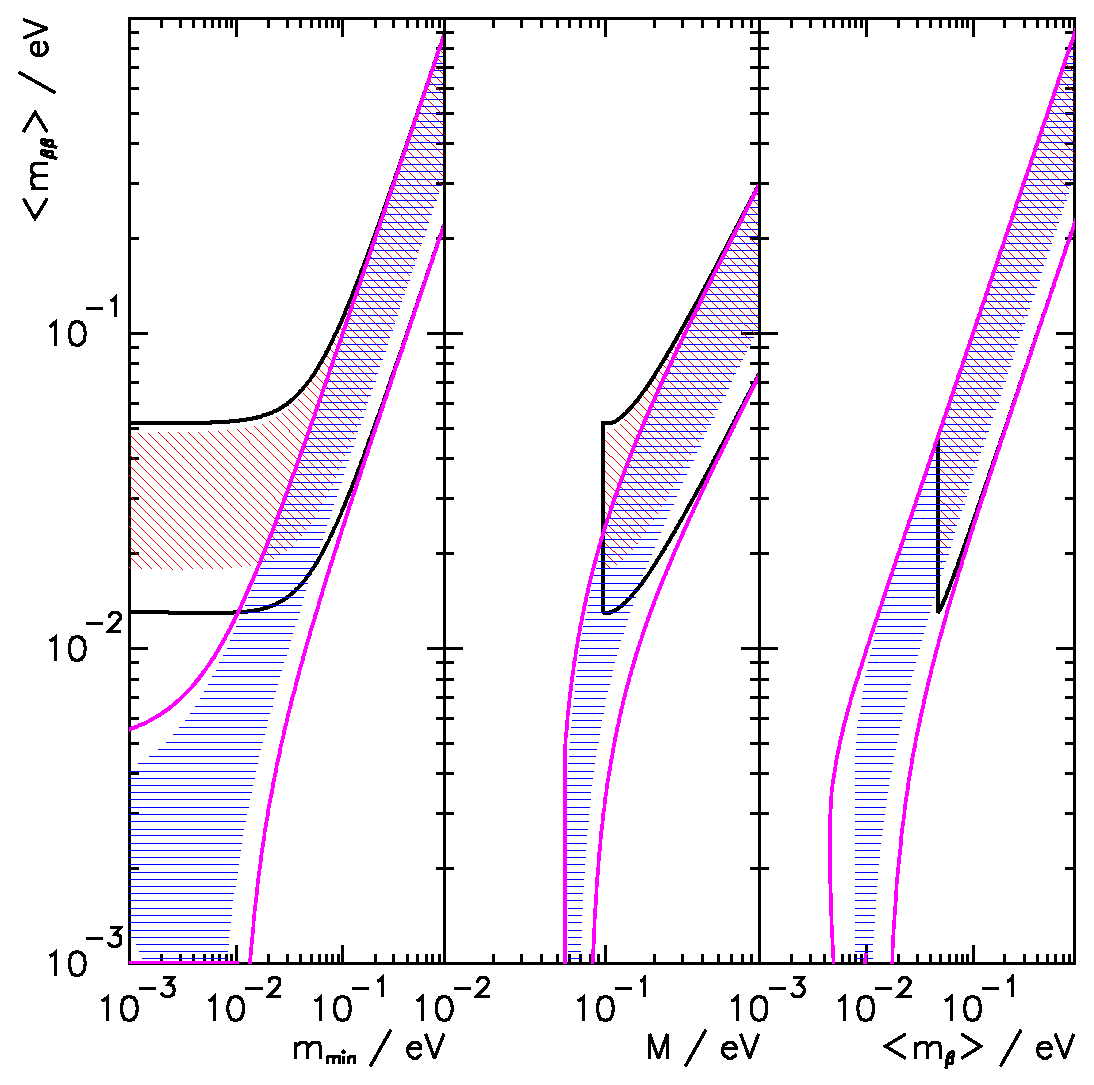
\includegraphics[keepaspectratio=true,width=\textwidth]{PDGNeutrinoMassBounds.eps}
\end{center}
\caption{The relationship between the effective Majorana mass $\left<m_{\beta\beta}\right>$ and other fundamental neutrino quantities: the lightest neutrino mass eigenstate $m_{min}$, the sum of mass eigenstates $M = \sum m_i$, and the effective single-beta-decay neutrino mass $\left<m_{\beta}\right>$.  Black (magenta) lines indicate the allowed region for the inverted (normal) hierarchy; red (blue) hatches indicate uncertainty for the inverted (normal) hierarchy due to the unknown CP-violating and Majorana phases $\delta$, $\alpha_1$, and $\alpha_2$~\cite{PDG}.}
\label{fig:NeutrinoMassBounds}
\end{figure}

It is possible to relate the observables $\left< m_{\beta\beta} \right>$, $\left< m_\beta \right>$, and $M$ within the model for $\mathbf{U}$ of equation~\ref{eqn:LongDefinitionOfU}.  These relations are shown in figure~\ref{fig:NeutrinoMassBounds}; we recall from section~\ref{sec:ParticlePhysicsConstraints} that beta spectrum measurements constrain $\left<m_\beta\right> < 2.05$ eV and cosmological observations constrain $M < 0.230$ eV, both with $90\%$ confidence.  The strongest constraints on $\left<m_{\beta\beta}\right>$ from $\beta\beta 0\nu$ searches place $\left<m_{\beta\beta}\right> < 0.15-0.4$ eV, depending on the choice of matrix element calculations.  We can see that if the cosmological limits are to be trusted, they provide the strongest constraints on the neutrino mass parameters; however, all three observables are complementary, and the wide range of experimental approaches means that systematic effects are unlikely to be shared by all three methods.

The sensitivity of an experiment for measuring $T_{1/2}^{0\nu}$ can be described by the approximate formula:~\cite{RMPbb0n}
\begin{equation}\label{eqn:ApproxHalflifeSensitivity}
T_{1/2}^{0\nu}(n_\sigma) = \frac{4.16 \cdot 10^{26} yrs}{n_\sigma} \left( \frac{\epsilon a}{W}\right) \sqrt{\frac{Mt}{b \Delta E}},
\end{equation}
where $M$ is the mass of material, $a$ is the isotopic enrichment, $W$ is the molecular mass of the material in atomic units, and $t$ is the live-time of the experiment; $\epsilon$ is the signal efficiency, $b$ is the background rate (in counts per kg keV year, or some similar units), and $\Delta E$ is the energy resolution of the detector at the $Q$-value; and $n_\sigma$ is the desired confidence limit, in sigmas, where the standard $90\%$ confidence limit will require $n_\sigma = 1.64$.  The scaling of this equation is most accurate when the energy resolution is much smaller than the $Q$-value and the background is uniformly distributed in energy; however it roughly allows us to compare the sensitivity of different $\beta\beta 0\nu$ experiments.

What it tells us, broadly, is that we should prefer experiments for which:
\begin{itemize}
\item A large quantity of highly-enriched isotope can be obtained.
\item Signal detection is highly efficient.
\item Background contamination around the $Q$-value is small, and does not scale with detector mass.
\item Good energy resolution can be achieved.
\end{itemize}

Currently the leading choices of materials for $\beta\beta 0\nu$ searches are:~\cite{RMPbb0n}
\begin{description}
\item[$^{76}$Ge] has by far the best energy resolution of any material, around $3$ keV.  It is also possible to grow Germanium crystals with fairly low background, with $0.06$ counts/(kg keV year) having been demonstrated.  However, it is expensive to grow large, clean crystals of Germanium, and as a result it may not be a scalable material.  It also has a $Q$-value of only $2039$ keV, giving it one of the lowest phase factors among the popular isotopes.  GERDA is currently the leading experiment, with data-taking underway.
\item[$^{130}$Te] also has an excellent energy resolution around $7$ keV.  Its $Q$-value is also higher than $^{76}$Ge, at $2530$ keV.  TeO$_2$ crystals must be grown, though, so it may suffer from some of the same challenges of scalability as Germanium.  The CUORE experiment is expected to begin data-taking in 2014.
\item[$^{136}$Xe] has a comparatively modest energy resolution around $35-40$ keV.  However, Xenon stands out for its scalability: it is easy to enrich in centrifuges, easy to purify chemically due to its status as a noble element, and it is easy to construct large monolithic detectors because it can be used in a liquid or gaseous state.  Background rates of $1-2\cdot 10^{-3}$ counts/(kg keV year) have been demonstrated.  There are currently two leading experiments.  KamLAND-Zen is the larger experiment, containing $180$ kg of active $^{136}$Xe; however, it detects only scintillation, and as a result its resolution is roughly $100$ keV.  EXO-200 only contains roughly $80$ kg of active $^{136}$Xe, but it detects energy through both the scintillation and ionization modes, and as a result is able to achieve energy resolutions around $35-40$ keV.
\end{description}

\begin{table}
\begin{center}
\begin{tabular}{|rccr|}
\hline Isotope & $T_{1/2}^{0\nu}$ (years, $90\%$ CL) & $\left<m_{\beta\beta}\right>$ (eV, $90\%$ CL) & Collaboration \\ \hline
$^{48}$Ca & $5.8 \cdot 10^{22}$ & $3.7$ & ELEGANT IV \cite{ElegantIV}\\
$^{76}$Ge & $2.1 \cdot 10^{25}$ & $0.24$ & GERDA \cite{PhysRevLett.111.122503} \\
$^{82}$Se & $3.6 \cdot 10^{23}$ & $1.1$ & NEMO-3 \cite{NEMO2011RandomOtherIsotopes}\\
$^{96}$Zr & $9.2 \cdot 10^{21}$ & $8.0$ & NEMO-3 \cite{Argyriades2010168}\\
$^{100}$Mo & $1.1 \cdot 10^{24}$ & $0.56$ & NEMO-3 \cite{NEMO3-2013-100Mo}\\
$^{116}$Cd & $1.6 \cdot 10^{22}$ & $6.1$ & NEMO-3 \cite{NEMO2011RandomOtherIsotopes}\\
$^{130}$Te & $3.0 \cdot 10^{24}$ & $0.34$ & Cuoricino \cite{PhysRevC.78.035502}\\
$^{136}$Xe & \textcolor{red}{FILL IN} & & \\
$^{136}$Xe & $1.9 \cdot 10^{25}$ & $0.16$ & KamLAND-Zen \cite{PhysRevLett.110.062502}\\
$^{150}$Nd & $1.8 \cdot 10^{22}$ & $3.4$ & NEMO-3 \cite{PhysRevC.80.032501}\\
\hline
\end{tabular}
\end{center}
\caption{A listing of the strongest available $\beta\beta 0\nu$ limits; all limits are quoted at $90\%$ confidence.  Limits on $\left<m_{\beta\beta}\right>$ are obtained using phase space factors from~\cite{PhysRevC.85.034316} and matrix elements from~\cite{PhysRevLett.109.042501}, both chosen for the completeness of their tabulations.  For $^{136}$Xe, both Kamland-Zen's published results and the EXO-200 results described in this work are included in the table.}
\label{tab:0nubb_limits}
\end{table}

Table~\ref{tab:0nubb_limits} tabulates the most current $T_{1/2}^{0\nu}$ limits in all $\beta\beta 0\nu$ isotopes for which $\beta\beta 0\nu$ limits have been published.  Representative limits on $\left< m_{\beta\beta}\right>$ are also included; these come from one particular set of phase space factors and nuclear matrix element calculations chosen because they have been tabulated for a broad range of isotopes and permit comparisons across all available half-life limits~\cite{PhysRevC.85.034316,PhysRevLett.109.042501}.  However, it should be remembered that errors in the matrix elements may propagate to errors in $\left< m_{\beta\beta}\right>$ of as much as a factor of two for each isotope.  We can see that although there are a favored set of isotopes, active and successful programs exist in a wide range of isotopes, and no one isotope is ideal in all respects.

As the table indicates, $^{136}$Xe has provided some of the strongest constraints on $\left< m_{\beta\beta}\right>$ in spite of its relatively modest energy resolution.  The present work will demonstrate that it is possible, in the EXO-200 detector, to produce significant improvements to the energy resolution through offline denoising of the scintillation signals.  This denoising technique will be applied to data from the detector, and will result in a stronger limit on $T_{1/2}^{0\nu}$ from EXO-200 than could be obtained from the same data without denoising.  Recent results will be presented which benefit from this and other improvements, as well as increased livetime.
